% \pdfoutput=1
% Uncomment line above if submitting to arXiv and using pdflatex

% $Id: main.tex 33041 2013-03-25 16:12:53Z tgershon $
% ============================================================================
% Purpose: Template for LHCb documents
% Authors: Tomasz Skwarnicki, Roger Forty, Ulrik Egede
% Created on: 2010-09-24
% ============================================================================
\documentclass[12pt,a4paper]{article}
% For two column text, add "twocolumn" as an option to the document
% class. Also uncomment the two "onecolumn" and "twocolumn" lines
% around the title page below.

% Variables that controls behaviour
\usepackage{ifthen} % for conditional statements
\usepackage{subfigure}
\usepackage[margin=2.5cm]{geometry}
\usepackage[T1]{fontenc}
\usepackage[utf8]{inputenc}
\usepackage{lmodern}
\usepackage{amsmath}
\usepackage{amssymb}
\usepackage{booktabs}
\usepackage{hyperref}
\usepackage{enumitem}
\usepackage{mdframed}

% All optional implementation prose is enclosed only by
% \begin{technicaldetails} ... \end{technicaldetails}.  Removing those two
% markers restores ordinary text; changing this definition restyles every
% technical block consistently.
\newmdenv[
  linecolor=technicalgray,
  linewidth=1.2pt,
  topline=false,
  rightline=false,
  bottomline=false,
  innerleftmargin=10pt,
  innerrightmargin=0pt,
  innertopmargin=5pt,
  innerbottommargin=5pt,
  skipabove=8pt,
  skipbelow=8pt,
  frametitle={Technical details (optional)},
  frametitlefont=\small\bfseries\color{technicalgray},
  frametitleaboveskip=0pt,
  frametitlebelowskip=4pt,
  repeatframetitle=false
]{technicaldetails}

\usepackage[abs]{overpic}
\setlength\unitlength{1mm}

\newboolean{pdflatex}
%\setboolean{pdflatex}{False} % False for eps figures 

%\newboolean{articletitles}
%\setboolean{articletitles}{true} % False removes titles in references

\newboolean{uprightparticles}
\setboolean{uprightparticles}{false} %True for upright particle symbols

%\newboolean{inbibliography}
%\setboolean{inbibliography}{false} %True once you enter the bibliography

\input{preamble}
\definecolor{technicalgray}{gray}{0.45}
%\usepackage{longtable} % only for template; not usually to be used in PAPERs

\begin{document}

%%%%%%%%%%%%%%%%%%%%%%%%%
%%%%% Title     %%%%%%%%%
%%%%%%%%%%%%%%%%%%%%%%%%%
\renewcommand{\thefootnote}{\fnsymbol{footnote}}
\setcounter{footnote}{1}

% \usepackage{lineno}
% \linenumbers*[1]

% %%%%%%% CHOOSE TITLE PAGE--------
%\onecolumn
% $Id: title-SHiP-NOTE.tex 14593 2012-01-27 14:43:32Z uegede $
% ===============================================================================
% Purpose: SHiP Public note title page template
% Author: 
% Created on: 2010-10-05
% ===============================================================================

%%%%%%%%%%%%%%%%%%%%%%%%%
%%%%%  TITLE PAGE  %%%%%%
%%%%%%%%%%%%%%%%%%%%%%%%%
\begin{titlepage}

\pagenumbering{roman}

% Header ---------------------------------------------------
\vspace*{-2.5cm}
\centerline{\large EUROPEAN ORGANIZATION FOR NUCLEAR RESEARCH (CERN)}
\vspace*{0.2cm}
\newcommand{\shiplogobox}{%
  \IfFileExists{SHiP-logo.pdf}{%
    
\includegraphics[width=0.15\linewidth]{SHiP-logo.pdf}%
  }{%
    \IfFileExists{SHiP-logo.eps}{%
      
\includegraphics[width=0.15\linewidth]{SHiP-logo.eps}%
    }{}%
  }%
}
\hspace*{-15mm}\begin{tabular*}{16.5cm}{lc@{\extracolsep{\fill}}r}
\vspace*{-10mm}\mbox{\shiplogobox}& & \\
 & & CERN-SHiP-NOTE-2026-CDS number \\  % ID 
 & & \today \\ % Date - Can also hardwire e.g.: 23 March 2010
% & & \\
\hline
\end{tabular*}

\vspace*{4.0cm}

% Title --------------------------------------------------
{\bf\boldmath\huge
\begin{center}
  UBT standalone simulation and FairShip implementation
\end{center}
}

\vspace*{2.0cm}

% Authors -------------------------------------------------
\begin{center}
V. Kholoimov$^1$
\bigskip\\
{\it\footnotesize
$^1$EPFL\\
}
\end{center}

\vspace{\fill}

% Abstract -----------------------------------------------
\begin{abstract}
\noindent
This note describes a standalone Geant4 model and its integration into
FairShip for the SHiP upstream background tagger (UBT).  The standalone
application simulates scintillation production and optical-photon transport
in \(40\times40\times10~\mathrm{mm^3}\) and
\(20\times20\times5~\mathrm{mm^3}\) tiles coupled to the same
\(6\times6~\mathrm{mm^2}\) photosensor. Position-dependent ADC/MeV maps derived from
the two tile configurations are used as compact calibration inputs to the
FairShip digitizer, avoiding optical-photon propagation during full detector
simulation.

The FairShip implementation constructs coarse \(40\times40~\mathrm{cm^2}\)
sensitive regions from a common YAML detector map.  During digitization, each
Monte Carlo point is assigned to the center of an implicit \(2\times2\) or
\(4\times4~\mathrm{cm^2}\) constituent tile.  Its deposited energy and exact
within-tile position determine the ADC count through the corresponding
response map, and a threshold of 100 ADC counts defines the trigger decision.
The note documents the geometry, physics assumptions, analysis workflow,
ROOT branches, calibration procedure, and current limitations.  In
particular, the simulated timing study remains preliminary and does not yet
reproduce real measurements; FairShip therefore currently uses a
real-data-based timing smearing rather than the simulated timing response.
\end{abstract}

\vspace*{2.0cm}
\vspace{\fill}

\end{titlepage}


% \pagestyle{empty}  % no page number for the title 

%%%%%%%%%%%%%%%%%%%%%%%%%%%%%%%%
%%%%%  EOD OF TInner TrackerLE PAGE  %%%%%%
%%%%%%%%%%%%%%%%%%%%%%%%%%%%%%%%

%  empty page follows the title page ----
% \newpage
% \setcounter{page}{2}
% \mbox{~}

% \cleardoublepage

%\input{title-SHiP-PROC}
%\input{title-SHiP-INT}
%\twocolumn
% %%%%%%%%%%%%% ---------

\renewcommand{\thefootnote}{\arabic{footnote}}
\setcounter{footnote}{0}

%%%%%%%%%%%%%%%%%%%%%%%%%%%%%%%%
%%%%%  Table of Content   %%%%%%
%%%%%%%%%%%%%%%%%%%%%%%%%%%%%%%%
%%%% Uncomment next 2 lines if desired
\tableofcontents
\cleardoublepage


%%%%%%%%%%%%%%%%%%%%%%%%%
%%%%% Main text %%%%%%%%%
%%%%%%%%%%%%%%%%%%%%%%%%%

\pagestyle{plain} % restore page numbers for the main text
\setcounter{page}{1}
\pagenumbering{arabic}

%% Uncomment during review phase. 
%% Comment before a final submission.
%\linenumbers

% You can include short sections directly in the main tex file.
% However, for larger papers it is desirable to split the text into
% several semiautonomous files, which can be revised independently.
% This is especially useful when developing a document in
% collaboration with several people, since then different parts can be
% edited independently.  This type of file organization is shown here.
% 
% \section{Introduction}
% \label{sec:Introduction}


% \begin{figure}[htb]
% \begin{center}
% 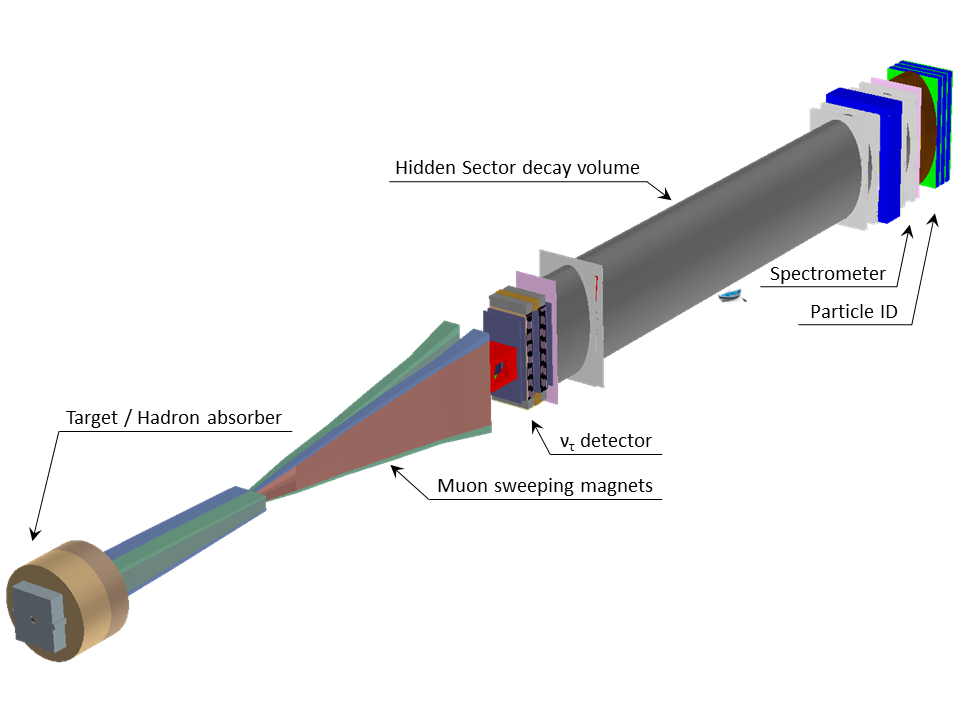
\includegraphics[width=0.8\linewidth]{figs/facility_layout.png}
% \caption{Overview of the SHiP experimental facility\cite{SHiP:TP}.}
% \label{fig:SHiP_overview}
% \end{center}
% \end{figure}

\section{Geometry}
\subsection{Volumes and Dimensions}
The geometry is defined in \texttt{src/DetectorConstruction.cc}. The world volume is an air box with half-size \texttt{(0.5 m, 0.5 m, 0.5 m)}. The active scintillator is a rectangular box with half-dimensions \texttt{(20 mm, 20 mm, 5 mm)}, corresponding to a full size of \texttt{40 x 40 x 10 mm$^{3}$}. The photosensor active transverse area is modeled with half-dimensions \texttt{(3 mm, 3 mm)}, corresponding to a full active face of \texttt{6 x 6 mm$^{2}$}.

Along the positive $z$ direction, the sensor stack is:
\begin{enumerate}[label=\arabic*.]
\item scintillator, ending at $z = +5~\mathrm{mm}$,
\item optical grease with thickness $0.2~\mathrm{mm}$,
\item glass window with thickness $1.0~\mathrm{mm}$,
\item photocathode / SiPM-sensitive slab with thickness $0.1~\mathrm{mm}$.
\end{enumerate}

All these volumes are centered on the same $x=y=0$ axis. The sensor is therefore mounted on the center of the $+z$ face of the scintillator.

\subsection{Coordinate Conventions}
The simulation uses the Geant4 global Cartesian system:
\begin{itemize}
\item the scintillator center is at $(0,0,0)$,
\item the beam propagates in the $+z$ direction,
\item the sensor stack is on the $+z$ side,
\item the muon source plane is upstream at negative $z$.
\end{itemize}

Primary hit positions stored in the output are the first recorded muon hit coordinates in the scintillator, in millimeters.

\subsection{Primary Generator Geometry}
The primary particle generator is defined in \texttt{src/PrimaryGeneratorAction.cc}. It uses a one-particle gun with:
\begin{itemize}
\item particle type: $\mu^-$,
\item initial position: $(0,0,-30~\mathrm{mm})$ by default,
\item momentum direction: $(0,0,1)$.
\end{itemize}

If position randomization is enabled, the initial $x$ and $y$ are sampled uniformly within a square beam spot:
\[
x, y \in [-a, +a],
\]
where $a$ is the configurable half-size. Internally, the member variable is initialized to $20~\mathrm{mm}$, while the UI messenger default string is currently set to $15~\mathrm{mm}$. This is a convention inconsistency that should be cleaned up.

Muon kinetic energy is sampled uniformly between
\[
1~\mathrm{GeV} \le E_\mu \le 20~\mathrm{GeV}.
\]

\section{Materials and Optical Properties}
\subsection{Scintillator Material}
The scintillator is modeled as an effective para-terphenyl + POPOP mixture with density
\[
\rho = 1.23~\mathrm{g/cm^3}.
\]
At the Geant4 material level, its bulk composition is still implemented as $\mathrm{C}_{18}\mathrm{H}_{14}$, that is, the host para-terphenyl stoichiometry. The POPOP admixture is represented through the emission spectrum rather than through an explicit dopant fraction in the material composition.

\subsection{Other Materials}
The remaining materials are:
\begin{itemize}
\item world: Geant4 air,
\item window: Geant4 Pyrex glass,
\item optical grease: simplified hydrocarbon material,
\item photocathode: simplified silicon slab.
\end{itemize}

\subsection{Emission Spectrum Convention}
The scintillation emission is specified as a tabulated relative spectrum versus photon energy. In the current implementation the table is:
\begin{center}
\begin{tabular}{cc}
\toprule
Photon energy [eV] & Relative intensity \\
\midrule
2.75 & 0.10 \\
2.85 & 0.55 \\
2.93 & 1.00 \\
3.00 & 0.75 \\
3.10 & 0.25 \\
\bottomrule
\end{tabular}
\end{center}

This is used for both \texttt{SCINTILLATIONCOMPONENT1} and \texttt{SCINTILLATIONCOMPONENT2}. Therefore, the fast and slow scintillation components differ only in time structure and relative yield, not in spectral shape.

These values are currently implemented as a compact approximation to the final blue emission expected from a para-terphenyl + POPOP scintillator, based on:
\begin{itemize}
\item Frontiers in Physics 12 (2024) 1289759, summarizing wavelength-shifted plastic-scintillator emission with a final band near $423~\mathrm{nm}$,
\item Journal of Spectroscopy (2012) 458126, reporting POPOP fluorescence near $415$--$416~\mathrm{nm}$ in solution.
\end{itemize}

The peak position is taken from the literature, while the exact five-point table is a compact hand-built Geant4 approximation rather than a digitized experimental spectrum. The implementation should therefore be understood as an effective mixed-emission model, not as a microscopic host-absorption / dopant-reemission simulation.

\subsection{Transport Properties}
The present optical properties are simplified:
\begin{itemize}
\item scintillator refractive index: constant at 1.58,
\item scintillator absorption length: constant at $210~\mathrm{cm}$,
\item grease refractive index: constant at 1.46,
\item glass refractive index: approximately 1.49--1.50,
\item photocathode refractive index: approximately 2.7--2.8,
\item grease absorption length: $500~\mathrm{cm}$,
\item glass absorption length: $300~\mathrm{cm}$,
\item photocathode absorption length: $10^{-6}~\mathrm{mm}$.
\end{itemize}

The very short photocathode absorption length is used as an efficient absorbing sink for photons that reach the sensitive surface.

\subsection{Surface Model}
Two optical surface conventions are used:
\begin{enumerate}[label=\arabic*.]
\item polished dielectric--dielectric interfaces between scintillator and grease, and between grease and window,
\item a diffuse wrapping skin surface on the scintillator with:
  \begin{itemize}
  \item reflectivity $R = 0.96$,
  \item \texttt{groundfrontpainted} finish,
  \item \texttt{unified} model,
  \item $\sigma_\alpha = 0.35$.
  \end{itemize}
\end{enumerate}

This wrapping model gives randomized reflected directions and introduces angular smearing at the boundaries.

\section{Scintillation Timing Model}
The timing constants are centralized in \texttt{include/TimingModelParameters.hh}. The current values are:
\begin{align*}
\tau_\mathrm{rise} &= 0.7~\mathrm{ns}, \\
\tau_\mathrm{fast} &= 2.0348~\mathrm{ns}, \\
\tau_\mathrm{slow} &= 11.3607~\mathrm{ns}, \\
Y_\mathrm{fast} &= 0.889145, \\
Y_\mathrm{slow} &= 0.110855.
\end{align*}

The total scintillation yield is set to
\[
10000~\mathrm{photons/MeV}.
\]

Finite rise time is enabled in the optical physics configuration. The same rise time is assigned to both scintillation components.

\section{Photon Detection Model}
\subsection{Boundary-Level Convention}
The PMT / SiPM sensitive detector acts only on optical photons crossing into the photocathode volume at a geometric boundary. This means the code does not simulate avalanche formation or analog waveform development. Instead, it applies two Bernoulli filters:
\begin{enumerate}[label=\arabic*.]
\item light-collection efficiency,
\item photon-detection efficiency.
\end{enumerate}

\subsection{Efficiencies}
In \texttt{src/PMTSensitiveDetector.cc}, the current values are:
\begin{align*}
\epsilon_\mathrm{LC} &= 0.30, \\
\epsilon_\mathrm{PDE} &= 0.64.
\end{align*}

The effective mean photoelectron conversion for photons that geometrically reach the sensor boundary is therefore
\[
\epsilon_\mathrm{eff} = \epsilon_\mathrm{LC}\,\epsilon_\mathrm{PDE} = 0.192.
\]

This is a strong simplification. In particular:
\begin{itemize}
\item \(\epsilon_\mathrm{LC}\) is applied as a random kill even after geometric transport has already occurred,
\item \(\epsilon_\mathrm{PDE}\) is wavelength-independent,
\item neither angle dependence nor fill factor is modeled explicitly,
\item no crosstalk, afterpulsing, recovery, or dark counts are included.
\end{itemize}

\section{Digitization Conventions}
\subsection{Charge Model}
Digitization is handled in \texttt{src/ScintillatorDigitizerModule.cc}. The number of detected photoelectrons is converted into charge through:
\[
Q = N_\mathrm{pe} \cdot G \cdot e,
\]
with
\begin{align*}
G &= 2.8 \times 10^6, \\
e &= 1.602176634 \times 10^{-19}\,\mathrm{C}.
\end{align*}

The code stores the charge in picocoulombs and uses
\[
\mathrm{ADC} = \mathrm{round}(Q[\mathrm{pC}]).
\]
Thus, the present ADC calibration is simply one ADC count per pC.

\subsection{Trigger Convention}
The trigger decision requires both:
\begin{itemize}
\item deposited energy above $0.20~\mathrm{MeV}$,
\item PMT charge above $5~\mathrm{pC}$.
\end{itemize}

\subsection{Time Reference Conventions}
Several different time references are used, and these are important:
\begin{enumerate}[label=\arabic*.]
\item \textbf{Absolute Geant4 global times}: used internally for photon births and arrivals.
\item \textbf{Times from primary hit}: for arrival-threshold observables and stored photoelectron arrival columns, times are shifted by the earliest recorded primary hit time in the scintillator.
\item \textbf{First PMT hit time}: stored in absolute nanoseconds.
\end{enumerate}

The function named \texttt{SetThreshold80TimeFromPrimary} currently stores the threshold-\(5\) photoelectron time from the muon hit. The data content is correct, but the naming is legacy and should be fixed.

\section{ROOT Output Conventions}
\subsection{Main Trees}
The code writes three ntuples:
\begin{enumerate}[label=\arabic*.]
\item \texttt{events},
\item \texttt{pmt\_photon\_births},
\item \texttt{scintillation\_photon\_birth\_times}.
\end{enumerate}

\subsection{Special Rows in \texttt{events}}
The \texttt{events} tree contains both physical events and synthetic summary rows:
\begin{itemize}
\item \texttt{event\_id = -1}, \texttt{primary\_particle = "RUN\_SUMMARY"},
\item \texttt{event\_id = -2}, \texttt{primary\_particle = "THRESHOLD\_SCAN"}.
\end{itemize}

This is convenient for quick downstream analysis, but it mixes different semantic object types inside one tree. Analyses must explicitly filter these rows.

\subsection{Stored Arrival-Time Columns}
The event tree stores photoelectron arrival times from the muon-hit reference for the following PE indices:
\[
1, 2, 3, 4, 5, 10, 20, 30, 40, 50, 60, 70, 80, 90, 100, 120, 140, 160, 180, 200.
\]

The naming convention is:
\[
\texttt{photoelectron\_arrival\_<N>\_from\_muon\_ns}.
\]

Unavailable values are written as \(-1\).

\subsection{Incident Photon Records}
The \texttt{pmt\_photon\_births} tree stores, for each photon that reached the sensor boundary:
\begin{itemize}
\item event ID,
\item birth position \((x,y,z)\),
\item birth time,
\item arrival time.
\end{itemize}

Internally these records are stored as
\[
\{x, y, z, t_\mathrm{birth}, t_\mathrm{arrival}\}.
\]

\section{Advantages of the Current Implementation}
\begin{enumerate}[label=\arabic*.]
\item \textbf{Simple and transparent geometry.} The model is easy to read and modify.
\item \textbf{Centralized timing constants.} Rise, fast, and slow components are stored in one header and reused by the timing validation tools.
\item \textbf{Good analysis visibility.} The code stores not only event-level summary quantities but also photon birth and arrival information.
\item \textbf{Fast iteration.} The simplified detection model is cheap to run and practical for scans.
\item \textbf{Direct threshold studies.} The stored photoelectron arrival columns are useful for timing-vs-threshold analysis.
\end{enumerate}

\section{Limitations and Drawbacks}
\begin{enumerate}[label=\arabic*.]
\item \textbf{Double simplification of light collection.} Optical transport is simulated, but an additional stochastic ``light collection efficiency'' cut is also applied at the sensor. This mixes geometric and phenomenological losses.
\item \textbf{Wavelength-independent PDE.} The photosensor response does not depend on wavelength, although the emission spectrum now does.
\item \textbf{No explicit host-to-dopant re-emission chain.} The present scintillator now uses an effective p-terphenyl + POPOP final emission spectrum, but it still does not simulate absorption by POPOP followed by delayed re-emission.
\item \textbf{No explicit surface roughness study beyond one wrap model.} The interface finishes are fixed and not experimentally tuned.
\item \textbf{Very simplified electronics.} Charge is proportional only to \(N_\mathrm{pe}\), with no single-photoelectron gain spread, noise, shaping, saturation, or baseline effects.
\end{enumerate}

\section{Most Useful Improvements}
The following upgrades would provide the largest gain in realism:
\begin{enumerate}[label=\arabic*.]
\item Replace the current compact effective emission approximation with a digitized measured p-terphenyl + POPOP spectrum.
\item If wavelength shifting is important, implement explicit POPOP absorption and re-emission rather than only the final effective emission band.
\item Replace the constant PDE with a wavelength-dependent PDE curve for the actual SiPM model.
\item Remove or reinterpret the extra \(\epsilon_\mathrm{LC}\) Bernoulli cut so that geometry and phenomenological losses are not counted ambiguously.
\item Introduce gain fluctuations, dark counts, and optionally waveform-level digitization if charge-width comparisons are important.
\item Separate event rows and run-summary rows into different trees or metadata objects.
\item Harmonize variable names, especially threshold-related naming.
\item Make the muon beam-spot default value consistent between the internal variable and the UI default string.
\end{enumerate}

\section{Summary}
The present implementation is a useful intermediate model: it contains full Geant4 optical transport through a realistic small detector geometry, but it still uses a deliberately simplified sensor and electronics model. This makes it practical for timing studies and fast iteration, while also making clear where phenomenological tuning enters the chain.

For timing scans and geometry studies, the current model is already informative. For quantitative comparison to measured charge spectra, wavelength-shifted emission, or realistic SiPM response, additional work is still needed.


\section{Conclusions}
\label{sec:conclusions}

The conclusions of this note are the following.



\begin{thebibliography}{999}
\bibitem{SHiP:EOI} 
W. Bonivento et al., \emph{Proposal to Search for Heavy Neutral Leptons at the
SPS}, October 2013, arXiv:130.1762v1.
\\
\bibitem{SHiP:TP} 
The SHiP Collaboration, \emph{Technical Proposal. An Experiment to Search for Hidden Particles (SHiP)
at the SPS}, CERN-SPSC-2015-016, SPSC-P-350, 8 April 2015.   
\\

\bibitem{SHiP:PP}
Alekhin, S. et al., Search for Hidden Particles, 
  CERN-SPSC-2015-017, SPSC-P-350-ADD-1, 9 April 2015. 
\\

\bibitem{SHiP:TPadd} 
The SHiP Collaboration, \emph{Addendum to Technical Proposal. An Experiment to Search for Hidden Particles (SHiP)
at the SPS}, CERN-SPSC-2015-040, SPSC-P-350-ADD-2, 19 October 2015
\\


\end{thebibliography}

%\begin{enumerate}
%
%\item Citations are marked using square brackets, and the
%  corresponding references should be typeset using Bib\TeX\ and the
%  official \lhcb Bib\TeX\ style. An example is in
%  Ref.~\cite{Sjostrand:2006za}.

%\item For references with four or less authors all of the authors'
%  names are listed~\cite{Majorana:1937vz}, otherwise the first author
%  is given, followed by \etal. The \lhcb Bib\TeX\ style will
%  take care of this.

%\item The order of references should be sequential when reading the
%  document. This is automatic when using Bib\TeX.

%\item The titles of papers should in general be included. To remove
%  them, change \texttt{\textbackslash
%    setboolean\{articletitles\}\{false\}} to \texttt{true} at the top
% of this template.

%\end{enumerate}

%There is a set of standard references to be used in \lhcb that are
%listed in Appendix~\ref{sec:StandardReferences}.


% This should be taken out in the final paper
%\input{supplementary-app}

%\addcontentsline{toc}{section}{References}
%\setboolean{inbibliography}{true}
%\bibliographystyle{LHCb}
%\bibliography{main,LHCb-PAPER,LHCb-CONF,LHCb-DP}

\end{document}
